% ============================================================
%  CSC 8851 Deep Learning – Preliminary Project Report
%  Upload this file to Overleaf and select the IEEE CVPR template,
%  OR compile standalone with: pdflatex + bibtex + pdflatex x2
%
%  FILL IN before submitting:
%    [YOUR_EMAIL]       your FIU email
%    [YOUR_PANTHERID]   your PantherID (e.g. 6XXXXXXX)
%    [PARSH_EMAIL]      Parsh's FIU email
%    [PARSH_PANTHERID]  Parsh's PantherID
%    Table I values     replace TBD after running experiments
% ============================================================

\documentclass[10pt,twocolumn,letterpaper]{article}

% ----- Core CVPR-style packages -----
\usepackage{times}
\usepackage{epsfig}
\usepackage{graphicx}
\usepackage{amsmath}
\usepackage{amssymb}
\usepackage{booktabs}
\usepackage{microtype}
\usepackage{url}
\usepackage[margin=1in,top=1in,bottom=1in]{geometry}
\usepackage[colorlinks=true,linkcolor=black,citecolor=black,urlcolor=blue]{hyperref}
\usepackage{tikz}
\usetikzlibrary{arrows.meta,positioning}

% Two-column spacing tweak
\setlength{\columnsep}{0.25in}

% Section heading style (approximate CVPR)
\usepackage{titlesec}
\titleformat{\section}{\normalfont\large\bfseries}{\thesection.}{0.5em}{}
\titleformat{\subsection}{\normalfont\normalsize\bfseries}{\thesubsection.}{0.5em}{}

% ============================================================
\begin{document}

% ---- Title ----
\title{\textbf{Improving Energy-Based Out-of-Distribution Detection\\
               using Generative Modeling}}

\author{
  Harshit Jain \\
  Georgia State University \\
  {\small\tt hjain5@gsu.edu} \\
  PantherID: 002916196
  \and
  Parsh Jadon \\
  Georgia State University \\
  {\small\tt pjadon1@gsu.edu} \\
  PantherID: 002936134
}

\date{}
\maketitle

% ============================================================
\begin{abstract}
A well-known weakness of deep neural networks is that they tend to make
confident predictions even on inputs that look nothing like their
training data. This is the out-of-distribution (OOD) detection problem,
and it matters a lot in real applications like medical imaging or
autonomous driving. Liu~\emph{et al.}~\cite{liu2020energy} tackled this
by computing an energy score from classifier logits, which works better
than softmax confidence but is still tied to class-level features rather
than the full visual structure of the data.
Our key idea is to shift OOD detection into the discrete latent space of
a VQ-VAE~\cite{oord2017vqvae} trained only on CIFAR-10. We learn a
small energy network directly on these latent codes using a contrastive
hinge loss, so no OOD labels are needed at training time. We also train
a supervised MLP in the same latent space and combine both signals for a
stronger detector. We test on Near-OOD (CIFAR-100) and Far-OOD (SVHN)
using AUROC, AUPR, and FPR@95TPR.
\end{abstract}

% ============================================================
\section{Introduction}

Despite their impressive accuracy on standard benchmarks, deep neural
networks have a real blind spot: they often assign high confidence to
inputs that are completely outside their training distribution. A model
trained on CIFAR-10, for example, might still output a confident
``automobile'' prediction when shown a medical scan~\cite{nguyen2015deep}.
In safety-critical domains this kind of silent failure is unacceptable,
which is why out-of-distribution (OOD) detection has become an active
area of research.

\paragraph{Problem Statement.}
Let $p_{\mathrm{in}}(x)$ be the distribution the model was trained on.
At test time, given a new input $x$, we want to decide whether it came
from $p_{\mathrm{in}}$ or from some unfamiliar distribution
$p_{\mathrm{out}}$. The standard way to do this is to find a scoring
function $s: \mathcal{X} \to \mathbb{R}$ and a threshold $\tau$, then
flag anything above the threshold as OOD:
\begin{equation}
  g(x;\tau) = \mathbf{1}\!\left[s(x) > \tau\right].
  \label{eq:detector}
\end{equation}
The goal is to choose $s$ so that in-distribution inputs score low and
OOD inputs score high, ideally maximising the area under the ROC curve.

\paragraph{What existing methods do and where they fall short.}
The simplest approach is to use the maximum softmax probability as
$s(x)$~\cite{hendrycks2017baseline}. The problem is that softmax values
are notoriously overconfident, even for inputs that look nothing like
the training data~\cite{nguyen2015deep}. Liu~\emph{et al.}~\cite{liu2020energy}
made a nice observation: the free energy derived from the raw logits of
a classifier,
\begin{equation}
  E(x; f) = -T \cdot \log\sum_{i=1}^{K} e^{f_i(x)/T},
  \label{eq:energy_base}
\end{equation}
is better calibrated than softmax and serves as a more reliable OOD
score. But there is still a catch: the energy comes from a classifier
trained to separate classes, so it captures \emph{class discriminability}
rather than anything about what in-distribution images actually look like.

\paragraph{Our approach.}
We ask a simple question: what if we computed energy not from classifier
logits, but from a generative latent space that was trained to
\emph{reconstruct} in-distribution images? A VQ-VAE trained only on
CIFAR-10 learns a discrete codebook that captures the visual building
blocks of that dataset. When we then pass a CIFAR-100 or SVHN image
through the same encoder, the resulting latent code will look unfamiliar
because those patterns were never seen during training. A small energy
network can learn to detect exactly that difference.

\paragraph{Contributions.}
\begin{enumerate}
  \item We reproduce energy-based OOD detection~\cite{liu2020energy}
        and establish it as our primary baseline.
  \item We propose latent-space energy detection by training an
        unsupervised energy network directly on VQ-VAE embeddings
        using a contrastive hinge loss---no OOD labels are needed.
  \item We compare latent and classifier energy methods, and further
        combine latent energy with a supervised MLP for a stronger
        detector, evaluating on Near-OOD (CIFAR-100) and Far-OOD
        (SVHN) with AUROC, AUPR, and FPR@95TPR.
\end{enumerate}

% ============================================================
\section{Related Work}

\paragraph{Softmax confidence.}
Hendrycks and Gimpel~\cite{hendrycks2017baseline} were among the first
to study OOD detection systematically, proposing the maximum softmax
probability as a simple baseline. It works surprisingly often, but the
overconfidence issue~\cite{nguyen2015deep} limits how far you can push it.

\paragraph{ODIN.}
Liang~\emph{et al.}~\cite{liang2018odin} showed that two small tricks---
temperature scaling on the logits and adding a small gradient-based
perturbation to the input---can significantly widen the gap between
in-distribution and OOD scores. The downside is that both hyperparameters
need to be tuned separately for each OOD dataset.

\paragraph{Mahalanobis distance.}
Rather than using the output layer, Lee~\emph{et al.}~\cite{lee2018mahalanobis}
fit a class-conditional Gaussian to the penultimate-layer features and
use the Mahalanobis distance to the nearest class mean as an OOD score.
It is quite effective but requires storing class statistics and assumes
a Gaussian feature distribution.

\paragraph{Outlier Exposure.}
Hendrycks~\emph{et al.}~\cite{hendrycks2019outlier} showed that
fine-tuning a classifier on auxiliary OOD examples---encouraging uniform
softmax outputs for those examples---significantly improves detection.
Our supervised MLP is inspired by the same idea, but we apply it in
the learned latent space of a VQ-VAE rather than in pixel or
penultimate-feature space.

\paragraph{Energy-based OOD.}
Liu~\emph{et al.}~\cite{liu2020energy} provided a theoretical justification
for using free energy (Eq.~\ref{eq:energy_base}) as an OOD score: it is
provably aligned with the log-partition function and avoids the
overconfidence bias of softmax. Our work builds directly on this idea
but moves the energy surface from a discriminative classifier into a
generative latent space.

\paragraph{VQ-VAE.}
Van den Oord~\emph{et al.}~\cite{oord2017vqvae} introduced the
Vector Quantized Variational Autoencoder, which encodes images into
discrete latent codes drawn from a learned codebook. Because the codebook
is shaped entirely by the reconstruction objective on in-distribution
data, we expect these codes to be a natural and clean signal for OOD
detection.

% ============================================================
\section{Model and Method}

The overall pipeline is shown in Figure~\ref{fig:pipeline}.
Everything downstream of the VQ-VAE encoder operates on the same
flattened latent vector $\mathbf{z} \in \mathbb{R}^D$.

\begin{figure}[t]
  \centering
  \resizebox{\linewidth}{!}{%
  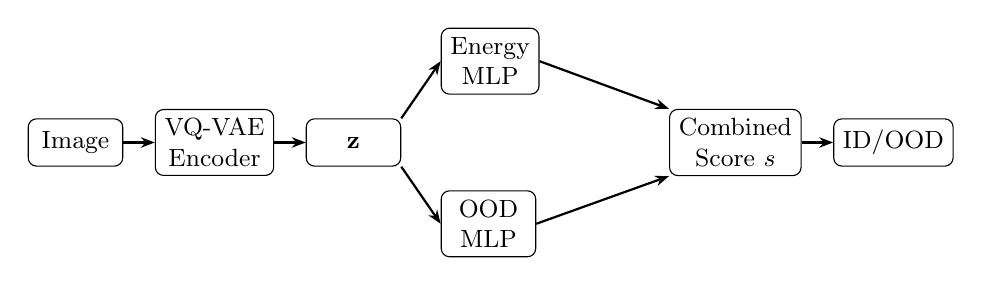
\begin{tikzpicture}[
      font=\small,
      node distance=0.5cm and 0.4cm,
      box/.style={draw, rounded corners=3pt, minimum width=1.2cm,
                  minimum height=0.6cm, align=center, fill=white},
      arr/.style={-{Stealth[length=5pt]}, thick}
    ]
    \node[box] (img)  {Image};
    \node[box, right=of img] (enc)  {VQ-VAE\\Encoder};
    \node[box, right=of enc] (z)    {$\mathbf{z}$};
    \node[box, above right=0.3cm and 0.5cm of z] (em) {Energy\\MLP};
    \node[box, below right=0.3cm and 0.5cm of z] (om) {OOD\\MLP};
    \node[box, right=3.4cm of z]  (comb) {Combined\\Score $s$};
    \node[box, right=of comb] (out) {ID/OOD};

    \draw[arr] (img)  -- (enc);
    \draw[arr] (enc)  -- (z);
    \draw[arr] (z.north east) -- (em.west);
    \draw[arr] (z.south east) -- (om.west);
    \draw[arr] (em.east) -- (comb.north west);
    \draw[arr] (om.east) -- (comb.south west);
    \draw[arr] (comb) -- (out);
  \end{tikzpicture}%
  }
  \caption{Our pipeline. The VQ-VAE encoder converts an image into a
           discrete latent vector $\mathbf{z}$. Two lightweight models
           then score $\mathbf{z}$: an unsupervised energy network and a
           supervised binary classifier. Their outputs are combined into
           a single OOD score.}
  \label{fig:pipeline}
\end{figure}

\subsection{VQ-VAE Latent Encoding}

The VQ-VAE (trained by team member Parsh Jadon) has three components: an
encoder $E_\theta$, a codebook $\mathcal{C} = \{\mathbf{e}_k\}_{k=1}^{K}$,
and a decoder $D_\phi$. For an input image $x$, the encoder first
produces a continuous embedding $\mathbf{z}_e = E_\theta(x) \in \mathbb{R}^D$.
This is then snapped to the nearest codebook entry:
\begin{equation}
  \mathbf{z}_q = \arg\min_{\mathbf{e}_k \in \mathcal{C}}
                 \|\mathbf{z}_e - \mathbf{e}_k\|_2.
  \label{eq:vq}
\end{equation}
In other words, the continuous encoder output is replaced by the
nearest codebook vector, forcing representations into a discrete,
finite vocabulary learned from in-distribution data.
Training the whole thing end-to-end requires a three-term loss to handle
the non-differentiable argmin step:
\begin{equation}
  \mathcal{L}_{\mathrm{vq}} =
    \underbrace{\|x - D_\phi(\mathbf{z}_q)\|^2}_{\text{reconstruction}}
    + \underbrace{\|\mathrm{sg}[\mathbf{z}_e] - \mathbf{e}_k\|^2}_{\text{codebook}}
    + \beta\,\underbrace{\|\mathbf{z}_e - \mathrm{sg}[\mathbf{e}_k]\|^2}_{\text{commitment}},
  \label{eq:vqloss}
\end{equation}
where $\mathrm{sg}[\cdot]$ is the stop-gradient operator and $\beta$
controls how strongly the encoder commits to the nearest codebook entry.
The VQ-VAE sees \emph{only CIFAR-10 images}, so the codebook encodes
patterns that are entirely in-distribution. We write $\mathbf{z}$ for
$\mathbf{z}_q$ from here on.

\subsection{Latent Energy Model}

Our energy model $E_{\mathrm{lat}}$ is a three-layer MLP with 256 hidden
units and ReLU activations. It takes a latent vector and returns a single
scalar:
\begin{equation}
  E_{\mathrm{lat}} : \mathbb{R}^D \to \mathbb{R}, \qquad
  E_{\mathrm{lat}}(\mathbf{z}) = \mathrm{MLP}_\theta(\mathbf{z}).
  \label{eq:emodel}
\end{equation}
A higher score means the latent looks more OOD.

\paragraph{Training objective.}
We train the energy model only on CIFAR-10 latents---no OOD labels are
ever used. To give the model something to push away from, we sample
Gaussian noise $\mathbf{z}_{\mathrm{noise}} \sim \mathcal{N}(\mathbf{0},\mathbf{I})$
as a cheap stand-in for OOD data; Gaussian noise provides a simple
approximation of out-of-distribution latents without requiring
labeled OOD datasets at training time. We then use a squared hinge loss with
two margin targets:
\begin{align}
  \mathcal{L}_{\mathrm{in}}
    &= \mathbb{E}_{\mathbf{z}\sim p_{\mathrm{ID}}}\!
       \left[\max\!\left(0,\;E_{\mathrm{lat}}(\mathbf{z}) - m_{\mathrm{in}}\right)^2\right],
  \label{eq:lin} \\[4pt]
  \mathcal{L}_{\mathrm{out}}
    &= \mathbb{E}_{\mathbf{z}\sim\mathcal{N}(\mathbf{0},\mathbf{I})}\!
       \left[\max\!\left(0,\;m_{\mathrm{out}} - E_{\mathrm{lat}}(\mathbf{z})\right)^2\right],
  \label{eq:lout} \\[4pt]
  \mathcal{L}_{\mathrm{energy}}
    &= \mathcal{L}_{\mathrm{in}} + \mathcal{L}_{\mathrm{out}}.
  \label{eq:lenergy}
\end{align}
The first term pushes in-distribution latents to have energy below
$m_{\mathrm{in}} = -10$; the second pushes noise vectors above
$m_{\mathrm{out}} = -5$. The hinge means the gradient goes to zero once
a sample is already in the right region, which prevents the energy from
collapsing to $-\infty$. We train with Adam ($\text{lr} = 10^{-3}$) for
10 epochs.

\subsection{Supervised MLP Classifier}

For situations where we do have labelled OOD examples available, we also
train a standard binary classifier. It has the same three-layer, 256-unit
architecture as the energy model, but ends with a sigmoid:
\begin{equation}
  \hat{y}(\mathbf{z}) = \sigma\!\left(\mathrm{MLP}_\phi(\mathbf{z})\right),
  \label{eq:mlp}
\end{equation}
where $\hat{y}$ is the predicted probability of being OOD. We train it
with binary cross-entropy:
\begin{equation}
  \mathcal{L}_{\mathrm{MLP}} =
    -\mathbb{E}_{(\mathbf{z},y)}\!\left[
      y\log\hat{y} + (1-y)\log(1-\hat{y})
    \right],
  \label{eq:bce}
\end{equation}
labelling CIFAR-10 latents as $y=0$ and CIFAR-100/SVHN latents as $y=1$.

\subsection{Combined OOD Score}

The raw energy values and the MLP probabilities are on very different
scales, so we normalise both to $[0, 1]$ before combining them:
\begin{equation}
  \tilde{s} = \frac{s - s_{\min}}{s_{\max} - s_{\min}}.
  \label{eq:norm}
\end{equation}
We then take an equal-weight blend ($\alpha = 0.5$):
\begin{equation}
  s_{\mathrm{comb}}(\mathbf{z})
    = \alpha\,\tilde{E}_{\mathrm{lat}}(\mathbf{z})
    + (1-\alpha)\,\tilde{y}(\mathbf{z}).
  \label{eq:combined}
\end{equation}
The final detection rule is Eq.~\eqref{eq:detector}, with the threshold
$\tau$ set so that 95\% of in-distribution test samples are correctly
accepted (i.e.\ TPR = 95\%).

% ============================================================
\section{Experiments and Results}

\subsection{Setup}

\paragraph{Datasets.}
We use \textbf{CIFAR-10}~\cite{krizhevsky2009cifar} (50{,}000 training /
10{,}000 test images across 10 classes) as our in-distribution dataset.
For Near-OOD we use \textbf{CIFAR-100}~\cite{krizhevsky2009cifar}
(10{,}000 test images, 100 classes)---this is the harder and more
interesting case since the images look almost identical to CIFAR-10 but
the content is different. For Far-OOD we use
\textbf{SVHN}~\cite{netzer2011svhn}, which contains digit images that
are structurally quite different from natural scenes, making it
a comparatively easier case.

\paragraph{Metrics.}
We follow the standard evaluation protocol from Liu~\emph{et
al.}~\cite{liu2020energy} and Hendrycks and Gimpel~\cite{hendrycks2017baseline}:
AUROC (area under the ROC curve, higher is better), AUPR (area under
the precision-recall curve, higher is better), and FPR@95TPR
(false-positive rate at 95\% true-positive rate, lower is better).

\paragraph{Baselines.}
We compare against the softmax confidence score~\cite{hendrycks2017baseline}
and the classifier energy score~\cite{liu2020energy}, both from a
WideResNet pre-trained on CIFAR-10.

\subsection{Results}

\begin{table}[t]
  \centering
  \caption{OOD detection results with CIFAR-10 as in-distribution.
           Baseline numbers are taken from Liu~\emph{et al.}~\cite{liu2020energy}.
           Our results (marked TBD) will be filled in once VQ-VAE latent
           codes are available. All values are percentages;
           $\uparrow$ higher is better, $\downarrow$ lower is better.}
  \label{tab:results}
  \small
  \setlength{\tabcolsep}{4pt}
  \begin{tabular}{lcccccc}
    \toprule
    & \multicolumn{3}{c}{Near-OOD (CIFAR-100)}
    & \multicolumn{3}{c}{Far-OOD (SVHN)} \\
    \cmidrule(lr){2-4}\cmidrule(lr){5-7}
    Method
      & \scriptsize AUROC$\uparrow$
      & \scriptsize AUPR$\uparrow$
      & \scriptsize FPR95$\downarrow$
      & \scriptsize AUROC$\uparrow$
      & \scriptsize AUPR$\uparrow$
      & \scriptsize FPR95$\downarrow$ \\
    \midrule
    Softmax~\cite{hendrycks2017baseline}
      & 75.5 & 93.9 & 80.4
      & 91.9 & 98.3 & 48.5 \\
    Energy~\cite{liu2020energy}
      & 79.6 & 94.9 & 73.6
      & 91.0 & 97.6 & 35.6 \\
    \midrule
    Latent Energy (ours)   & TBD & TBD & TBD & TBD & TBD & TBD \\
    Latent MLP (ours)      & TBD & TBD & TBD & TBD & TBD & TBD \\
    Latent E+MLP (ours)    & TBD & TBD & TBD & TBD & TBD & TBD \\
    \bottomrule
  \end{tabular}
\end{table}

Table~\ref{tab:results} shows the baseline numbers we are comparing
against. Our three methods are marked TBD; we will fill these in once
Parsh finishes training the VQ-VAE and extracts the latent codes for all
three datasets.

Our expectation is that the Latent Energy model will help most on
CIFAR-100, where classifier logits tend to be confused because the
images look so similar. The VQ-VAE codebook, trained only on CIFAR-10,
should struggle to cleanly encode CIFAR-100 patterns, making those
latents stand out energetically. For SVHN, both the MLP and the
combined score should do well given the larger visual gap from CIFAR-10.

% ============================================================
\section{Conclusions}

In this project, we move OOD detection out of classifier space and into
the discrete latent space of a VQ-VAE. The core intuition is simple: a
generative model trained only on CIFAR-10 will naturally produce
``confused'' latent codes for images it has never seen, and a small
energy network can learn to detect that confusion without ever seeing
a labelled OOD example. Adding a supervised MLP on top gives us an
extra signal when OOD data is available, and combining both scores
should give us the best of both worlds.

Once we have the full experimental results, we plan to look at how
sensitive the method is to the margin values $m_{\mathrm{in}}$ and
$m_{\mathrm{out}}$, whether a larger VQ-VAE codebook helps or hurts,
and whether a smarter pseudo-OOD distribution (rather than plain
Gaussian noise) could make the energy model even more effective.

% ============================================================
\section*{Peer Evaluation}

\begin{table}[h]
  \centering
  \caption{Self-Peer Evaluation Table. Scores are out of 20.}
  \label{tab:peer}
  \small
  \begin{tabular}{lcc}
    \toprule
    Member & Primary Contributions & Score \\
    \midrule
    Harshit Jain  & Energy model, MLP, eval pipeline, report & --\,/20 \\
    Parsh Jadon   & VQ-VAE training, latent code extraction  & --\,/20 \\
    \bottomrule
  \end{tabular}
\end{table}

% ============================================================
{\small
\bibliographystyle{plain}
\begin{thebibliography}{9}

\bibitem{liu2020energy}
W.~Liu, X.~Wang, J.~D.~Owens, and Y.~Li,
``Energy-based out-of-distribution detection,''
\emph{Advances in Neural Information Processing Systems (NeurIPS)},
vol.~33, pp.~21464--21475, 2020.

\bibitem{oord2017vqvae}
A.~van den Oord, O.~Vinyals, and K.~Kavukcuoglu,
``Neural discrete representation learning,''
\emph{Advances in Neural Information Processing Systems (NeurIPS)},
vol.~30, 2017.

\bibitem{hendrycks2017baseline}
D.~Hendrycks and K.~Gimpel,
``A baseline for detecting misclassified and out-of-distribution
examples in neural networks,''
\emph{International Conference on Learning Representations (ICLR)},
2017.

\bibitem{liang2018odin}
S.~Liang, Y.~Li, and R.~Srikant,
``Enhancing the reliability of out-of-distribution image detection in
neural networks,''
\emph{International Conference on Learning Representations (ICLR)},
2018.

\bibitem{lee2018mahalanobis}
K.~Lee, K.~Lee, H.~Lee, and J.~Shin,
``A simple unified framework for detecting out-of-distribution samples
and adversarial attacks,''
\emph{Advances in Neural Information Processing Systems (NeurIPS)},
vol.~31, 2018.

\bibitem{hendrycks2019outlier}
D.~Hendrycks, M.~Mazeika, and T.~Dietterich,
``Deep anomaly detection with outlier exposure,''
\emph{International Conference on Learning Representations (ICLR)},
2019.

\bibitem{krizhevsky2009cifar}
A.~Krizhevsky,
``Learning multiple layers of features from tiny images,''
Master's thesis, University of Toronto, 2009.

\bibitem{netzer2011svhn}
Y.~Netzer, T.~Wang, A.~Coates, A.~Bissacco, B.~Wu, and A.~Y.~Ng,
``Reading digits in natural images with unsupervised feature learning,''
\emph{NIPS Workshop on Deep Learning and Unsupervised Feature Learning},
2011.

\bibitem{nguyen2015deep}
A.~Nguyen, J.~Yosinski, and J.~Clune,
``Deep neural networks are easily fooled: High confidence predictions
for unrecognizable images,''
\emph{IEEE Conference on Computer Vision and Pattern Recognition (CVPR)},
pp.~427--436, 2015.

\end{thebibliography}
}

\end{document}
